\chapter{Arhitektura i dizajn sustava}
		
	% 	\textbf{\textit{dio 1. revizije}}\\

	% 	\textit{ Potrebno je opisati stil arhitekture te identificirati: podsustave, preslikavanje na radnu platformu, spremišta podataka, mrežne protokole, globalni upravljački tok i sklopovsko-programske zahtjeve. Po točkama razraditi i popratiti odgovarajućim skicama:}
	% \begin{itemize}
	% 	\item 	\textit{izbor arhitekture temeljem principa oblikovanja pokazanih na predavanjima (objasniti zašto ste baš odabrali takvu arhitekturu)}
	% 	\item 	\textit{organizaciju sustava s najviše razine apstrakcije (npr. klijent-poslužitelj, baza podataka, datotečni sustav, grafičko sučelje)}
	% 	\item 	\textit{organizaciju aplikacije (npr. slojevi frontend i backend, MVC arhitektura) }		
	% \end{itemize}
		
		\section{Organizacija sustava}
			\subsection{Uvod}
				Arhitekturu sustava čine tri glavna dijela:
				\begin{packed_item}
					\item Baza podataka
					\item Aplikacijski front-end
					\item Aplikacijski back-end
				\end{packed_item}
			
				Front-end aplikacije ključan je dio u uspostavljanju komunikacije između korisnika i aplikacije. Korisnik aplikaciji pristupa uz pomoć internetskog preglednika na svom računalu, mobitelu ili nekom drugom uređaju. Preglednik komunicira s poslužiteljem preko HTTP protokola slanjem odgovarajućih zahtjeva. Front-end korisnikove zahtjeve zatim prosljeđuje back-endu koji predstavlja samu aplikaciju.
				\linebreak
				Aplikacija preuzima zahtjev te ga obrađuje sukladno njegovoj vrsti i parametrima. Obrada zahtjeva uključuje i pristupanje bazi podataka kako bi se dohvatili podatci potrebni za rad. Po završetku obrade zahtjeva, aplikacija front-endu vraća odgovor, a on ga dalje šalje korisniku.
				\linebreak
				Baza podataka može se nalaziti na istom računalu kao i ostali dijelovi sustava ili različitom, no komunikacija se uvijek odvija na isti način, preko dobro poznatih vrata na transportnom sloju i korištenjem odgovarajućeg protokola.
				\begin{figure}[H]
					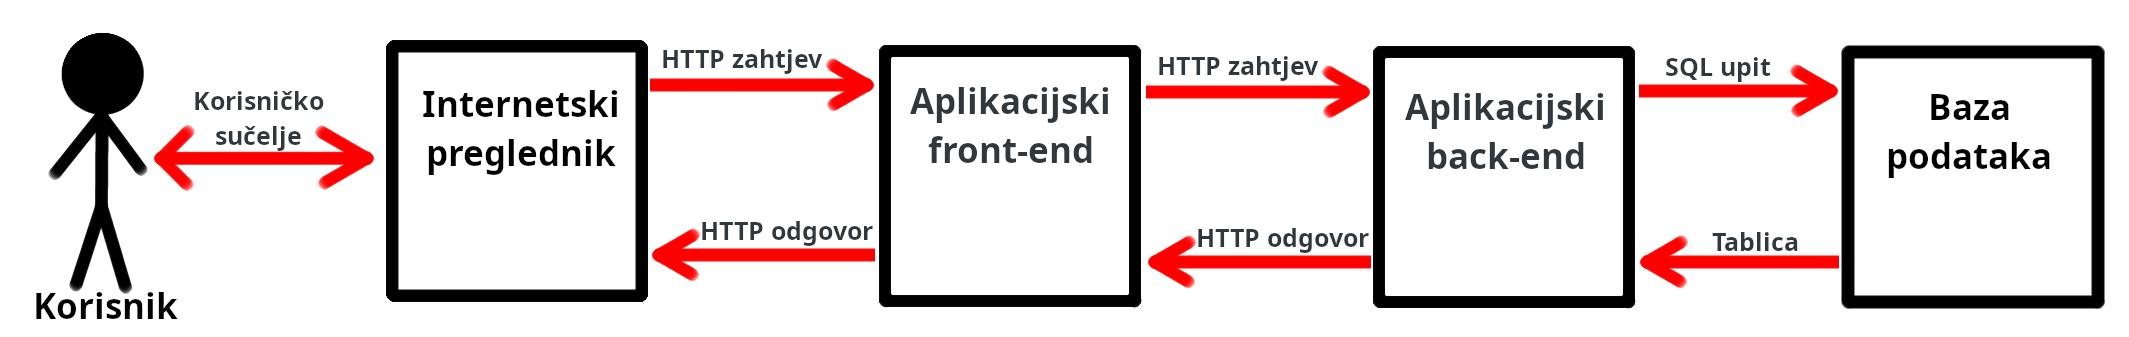
\includegraphics[scale=0.85]{slike/skica_arhitekture.png}
					\centering
					\caption{Arhitektura sustava}
					\label{fig:arhitektura_sustava}
				\end{figure}
			\subsection{Sklopovski zahtjevi}
				Ako se aplikacijski poslužitelj i baza podataka nalaze na različitim računalima, za optimalan rad ona bi trebala imati odgovarajuće karakteristike. Računalo na kojem će raditi poslužitelj treba imati dovoljnu veliku procesorsku moć kako bi moglo što brže odgovarati na zahtjeve i kako bi više korisnika moglo koristiti aplikaciju bez značajnog usporavanja sustava. Računalo na kojem će se nalaziti baza podataka treba imati dovoljno velike i brze diskove za pohranu podataka, idealno uz neku vrstu zaštite od gubitka podataka u slučaju kvara (na primjer, korištenje RAID sustava ili automatskog redovitog stvaranja sigurnosne kopije). Ako se pak poslužitelj i baza podataka pokreću na istom računalu, ono treba kombinirati maloprije navedene karakteristike.
			\subsection{Organizacija aplikacije}
				Za izradu aplikacije odabrani su programski jezik Java uz razvojni okvir Spring te Javascript i razvojni okvir React. Dva glavna sloja aplikacije su frontend, koji komunicira s korisnikom (Javascript + React) i backend, koji obrađuje HTTP zahtjeve i komunicira s bazom podataka (Java + Spring).
				%U primjeru dokumentacije oni ovdje jos pisu da se arhitektura temelji na MVCu i to dodatno opisuju
				%Ovaj dio bi onda trebali dovrsit kada vidimo sto cemo s time
				
				
		

				\section{Baza podataka}
			
				Naš će sustav koristiti relacijsku bazu podataka čija je osnovna jedinica baze relacija, odnosno tablica, koja je definirana svojim imenom i skupom atributa. Baza podataka ima zadatak brzo i jednostavno pohranjivati, mijenjati i dohvaćati podatke za daljnju obradu. Baza podataka stranice sastoji se od sljedećih entiteta:
				 \begin{packed_item}
					 \item Korisnik
					 \item Recept
					 \item Oznaka
						 \item Komentar
					 \item Ocjena
					 \item Poruka
						 \item Sastojak
				 \end{packed_item}
		 
			 \subsection{Opis tablica}
			 
 
				 \textbf{Korisnik} Ovaj entitet sadržava sve važne informacije o korisniku aplikacije. Sadrži atribute: Korisničko ime, lozinku, ime, prezime, broj mobitela korisnika, razinu ovlasti korisnika i e-mail korisnika. Ovaj entitet u vezi je \textit{One-to-Many} s entitetima Recept, Komentar i Ocjena te je s entitetom poruka u ulozi primatelj i pošiljatelj isto u \textit{One-to-Many} vezi, sve preko ID-a korisnika.
				 
				 
				 \begin{longtblr}[
					 label=none,
					 entry=none
					 ]{
						 width = \textwidth,
						 colspec={|X[8,l]|X[8, l]|X[18, l]|}, 
						 rowhead = 1,
					 } %definicija širine tablice, širine stupaca, poravnanje i broja redaka naslova tablice
					 \hline \SetCell[c=3]{c}{\textbf{Korisnik}}	 \\ \hline[3pt]
					 \SetCell{LightGreen} ID Korisnika	& INT &  jedinstveni identifikator korisnika\\ \hline 
					 Lozinka & VARCHAR	&  lozinka korisnika	\\ \hline 
						 Korisničko ime & VARCHAR	&  korisničko ime	\\ \hline 
						 Ime & VARCHAR	& ime korisnika\\ \hline 
					 Prezime & VARCHAR &  prezime korisnika \\ \hline 
						 Broj mobitela & VARCHAR	& telefonski broj korisnika\\ \hline 
						 Razina Ovlasti & VARCHAR &  razina ovlasti korisnika \\ \hline 
					 Email & VARCHAR & e-mail adresa korisnika 	\\ \hline 
				 \end{longtblr}
				 
				 \textbf{Recept} Ovaj entitet sadržava sve važne informacije o receptu. Sadrži atribute: ID recepta, naziv recepta, vrijeme pripreme, postupak pripreme, opis recepta, sliku recepta, datum recepta  i vrijeme objave recepta i prosječnu ocjenu recepta. Recept je u vezi \textit{Many-to-One} s korisnikom koji ga je objavio, u vezi \textit{One-to-Many} s ocjenom, sastojkom u receptu i komentarom preko ID-a recepta te u \textit{Many-to-Many} s oznakom recepta preko ID-a oznake.
				 
				 \begin{longtblr}[
					 label=none,
					 entry=none
					 ]{
						 width = \textwidth,
						 colspec={|X[8,l]|X[8, l]|X[18, l]|}, 
						 rowhead = 1,
					 } %definicija širine tablice, širine stupaca, poravnanje i broja redaka naslova tablice
					 \hline \SetCell[c=3]{c}{\textbf{Recept}}	 \\ \hline[3pt]
					 \SetCell{LightGreen}ID Recepta & INT	&  	jedinstveni identifikator recepta  	\\ \hline
					 Naziv recepta	& VARCHAR &   naziv recepta	\\ \hline 
					 Vrijeme pripreme & INTERVAL & vrijeme pripreme  \\ \hline 
					 Postupak pripreme & VARCHAR	& postupak pripreme\\ \hline 
					 Opis recepta & VARCHAR & opis recepta \\ \hline 
					 Slika recepta & LONGBOB	&  slika recepta	\\ \hline 
						 Datum i vrijeme recepta	& DATETIME & datum recepta  i vrijeme objave recepta 	\\ \hline 
						 Prosječna ocjena recepta	& INT &   prosječna ocjena recepta	\\ 
						 \hline
						 \SetCell{LightBlue} ID Korisnika	& INT &  ID korisnika koji je objavio recept\\ \hline 
						 \SetCell{LightBlue} ID oznake	& INT &  ID oznake recepta\\ \hline 
				 \end{longtblr}
 
				 \textbf{Oznaka} Ovaj entitet sadržava sve važne informacije o oznaci recepta. Sadrži atribute: ID oznake i naziv oznake. Oznaka je u \textit{Many-to-Many} vezi s receptom preko ID-a oznake.
	 
				 \begin{longtblr}[
					 label=none,
					 entry=none
					 ]{
						 width = \textwidth,
						 colspec={|X[8,l]|X[8, l]|X[18, l]|}, 
						 rowhead = 1,
					 } %definicija širine tablice, širine stupaca, poravnanje i broja redaka naslova tablice
					 \hline \SetCell[c=3]{c}{\textbf{Oznaka}}	 \\ \hline[3pt]
					 \SetCell{LightGreen}ID oznake & INT	&  	jedinstveni identifikator oznake  	\\ \hline
					 Naziv oznake & VARCHAR & naziv oznake  	\\ \hline 
				 \end{longtblr}
 
				 \textbf{Komentar} Ovaj entitet sadržava sve važne informacije o komentaru recepta. Sadrži atribute: ID komentara, ID komentatora, ID recepta, tekst komentara i datum i vrijeme komentara. Komentar je u \textit{Many-to-One} vezi s korisnikom preko ID-a korisnika koji ga objavi i receptom preko ID-a recepta. 
 
				 \begin{longtblr}[
					 label=none,
					 entry=none
					 ]{
						 width = \textwidth,
						 colspec={|X[8,l]|X[8, l]|X[18, l]|}, 
						 rowhead = 1,
					 } %definicija širine tablice, širine stupaca, poravnanje i broja redaka naslova tablice
					 \hline \SetCell[c=3]{c}{\textbf{Komentar}}	 \\ \hline[3pt]
						 \SetCell{LightGreen}ID komentar & INT &  ID komentara	\\ \hline
					 Tekst komentara	& VARCHAR &  tekst komentara 	\\ \hline 
						 ID komentatora	& INT &  ID korisnika komentatora	\\ \hline
						 ID recepta	& INT &  ID recepta na kojem je komentar postavljen	\\ \hline
						 Datum i vrijeme komentara	& DATETIME &  datum i vrijeme komentara	\\ \hline 
				 \end{longtblr}
 
				 \textbf{Ocjena} Ovaj entitet sadržava sve važne informacije o pojedinoj ocjeni recepta. Sadrži atribute: ID ocjenitelja, ID recepta i datum i vrijeme ocjene. Entitet je u vezi \textit{Many-to-One} s ocjeniteljem preko ID-a korisnika koji je ocijenio recept i \textit{Many-to-One} s receptom preko ID-a recepta.
 
				 \begin{longtblr}[
					 label=none,
					 entry=none
					 ]{
						 width = \textwidth,
						 colspec={|X[8,l]|X[8, l]|X[18, l]|}, 
						 rowhead = 1,
					 } %definicija širine tablice, širine stupaca, poravnanje i broja redaka naslova tablice
					 \hline \SetCell[c=3]{c}{\textbf{Ocjena}}	 \\ \hline[3pt]
					 Ocjena	& VARCHAR & ocjena	\\ \hline
						 \SetCell{LightBlue}ID ocjenitelja	& INT &  ID korisnika koji je ostavio poruku	\\ \hline
						 \SetCell{LightBlue}ID recepta	& INT &  ID recepta koji je ocjenjen	\\ \hline
						 Datum i vrijeme ocjene	& DATETIME &  datum i vrijeme ocjene	\\ \hline 
				 \end{longtblr}
 
				 \textbf{Poruka} Ovaj entitet sadržava sve važne informacije o poruci između dva korisnika. Sadrži atribute: ID poruke, ID pošiljatelja, ID primatelja, tekst poruke i datum i vrijeme poruke. Poruka je u vezi \textit{Many-to-One} s primateljem i pošiljateljem preko ID-a korisnika koji palje i prima poruku.
 
				 \begin{longtblr}[
					 label=none,
					 entry=none
					 ]{
						 width = \textwidth,
						 colspec={|X[8,l]|X[8, l]|X[18, l]|}, 
						 rowhead = 1,
					 } %definicija širine tablice, širine stupaca, poravnanje i broja redaka naslova tablice
					 \hline \SetCell[c=3]{c}{\textbf{Poruka}}	 \\ \hline[3pt]
						 \SetCell{LightGreen}ID Poruka	& INT &  ID poruka \\ \hline
					 Tekst poruka & VARCHAR & tekst poruka  	\\ \hline 
						 ID pošiljatelja	& INT &  ID korisnika koji šalje poruku	\\ \hline 
						 ID primatelja	& INT & ID korisnika koji prima poruku	\\ \hline 
						 Datum i vrijeme poruke & TIMESTAMP &  datum i vrijeme poruke	\\ \hline 
				 \end{longtblr}
 
				 \textbf{Sastojak} Ovaj entitet sadržava sve važne informacije o sastojku navedenom u nekom receptu. Sadrži atribute: ID sastojka, naziv sastojka. Entitet je u vezi \textit{Many-to-Many} sa sastojkom u receptu preko ID-a recepta.
 
				 \begin{longtblr}[
					 label=none,
					 entry=none
					 ]{
						 width = \textwidth,
						 colspec={|X[8,l]|X[8, l]|X[18, l]|}, 
						 rowhead = 1,
					 } %definicija širine tablice, širine stupaca, poravnanje i broja redaka naslova tablice
					 %Zašto imamo IDSastojak? Jer može biti više sastojaka s istim imenom, istom količinom u istom receptu (npr 100 ml mlijeka u kremi i 100 ml mlijeka u tjestu)
					 \hline \SetCell[c=3]{c}{\textbf{Sastojak}}	 \\ \hline[3pt]
						 \SetCell{LightGreen}ID Sastojka	& INT &  ID sastojka \\ \hline
						 Naziv sastojka	& VARCHAR &  naziv sastojka	\\ \hline
					 
				 \end{longtblr}
 
				 \textbf{Sastojak u receptu} Ovaj entitet sadržava sve važne informacije o sastojku navedenom u nekom receptu. Sadrži atribute: ID sastojka, ID recepta, količinu. Entitet je u vezi \textit{Many-to-One} s receptom preko ID-a recepta i u vezi \textit{Many-to-Many} sa sastojkom preko ID sastojak.
				 
				 \begin{longtblr}[
					 label=none,
					 entry=none
					 ]{
						 width = \textwidth,
						 colspec={|X[8,l]|X[8, l]|X[18, l]|}, 
						 rowhead = 1,
					 } %definicija širine tablice, širine stupaca, poravnanje i broja redaka naslova tablice
					 %Zašto imamo IDSastojak? Jer može biti više sastojaka s istim imenom, istom količinom u istom receptu (npr 100 ml mlijeka u kremi i 100 ml mlijeka u tjestu)
					 \hline \SetCell[c=3]{c}{\textbf{Sastojak u receptu}}	 \\ \hline[3pt]
						 \SetCell{LightBlue}ID Sastojka	& INT &  ID sastojka \\ \hline
						 \SetCell{LightBlue}ID recepta	& INT &   ID recepta u kojem je sastojak	\\ \hline
						 Količina	& VARCHAR &   količina	\\ \hline
					 
				 \end{longtblr}
				 
			 
			 \subsection{Dijagram baze podataka}
			 \begin{figure}[H]
				 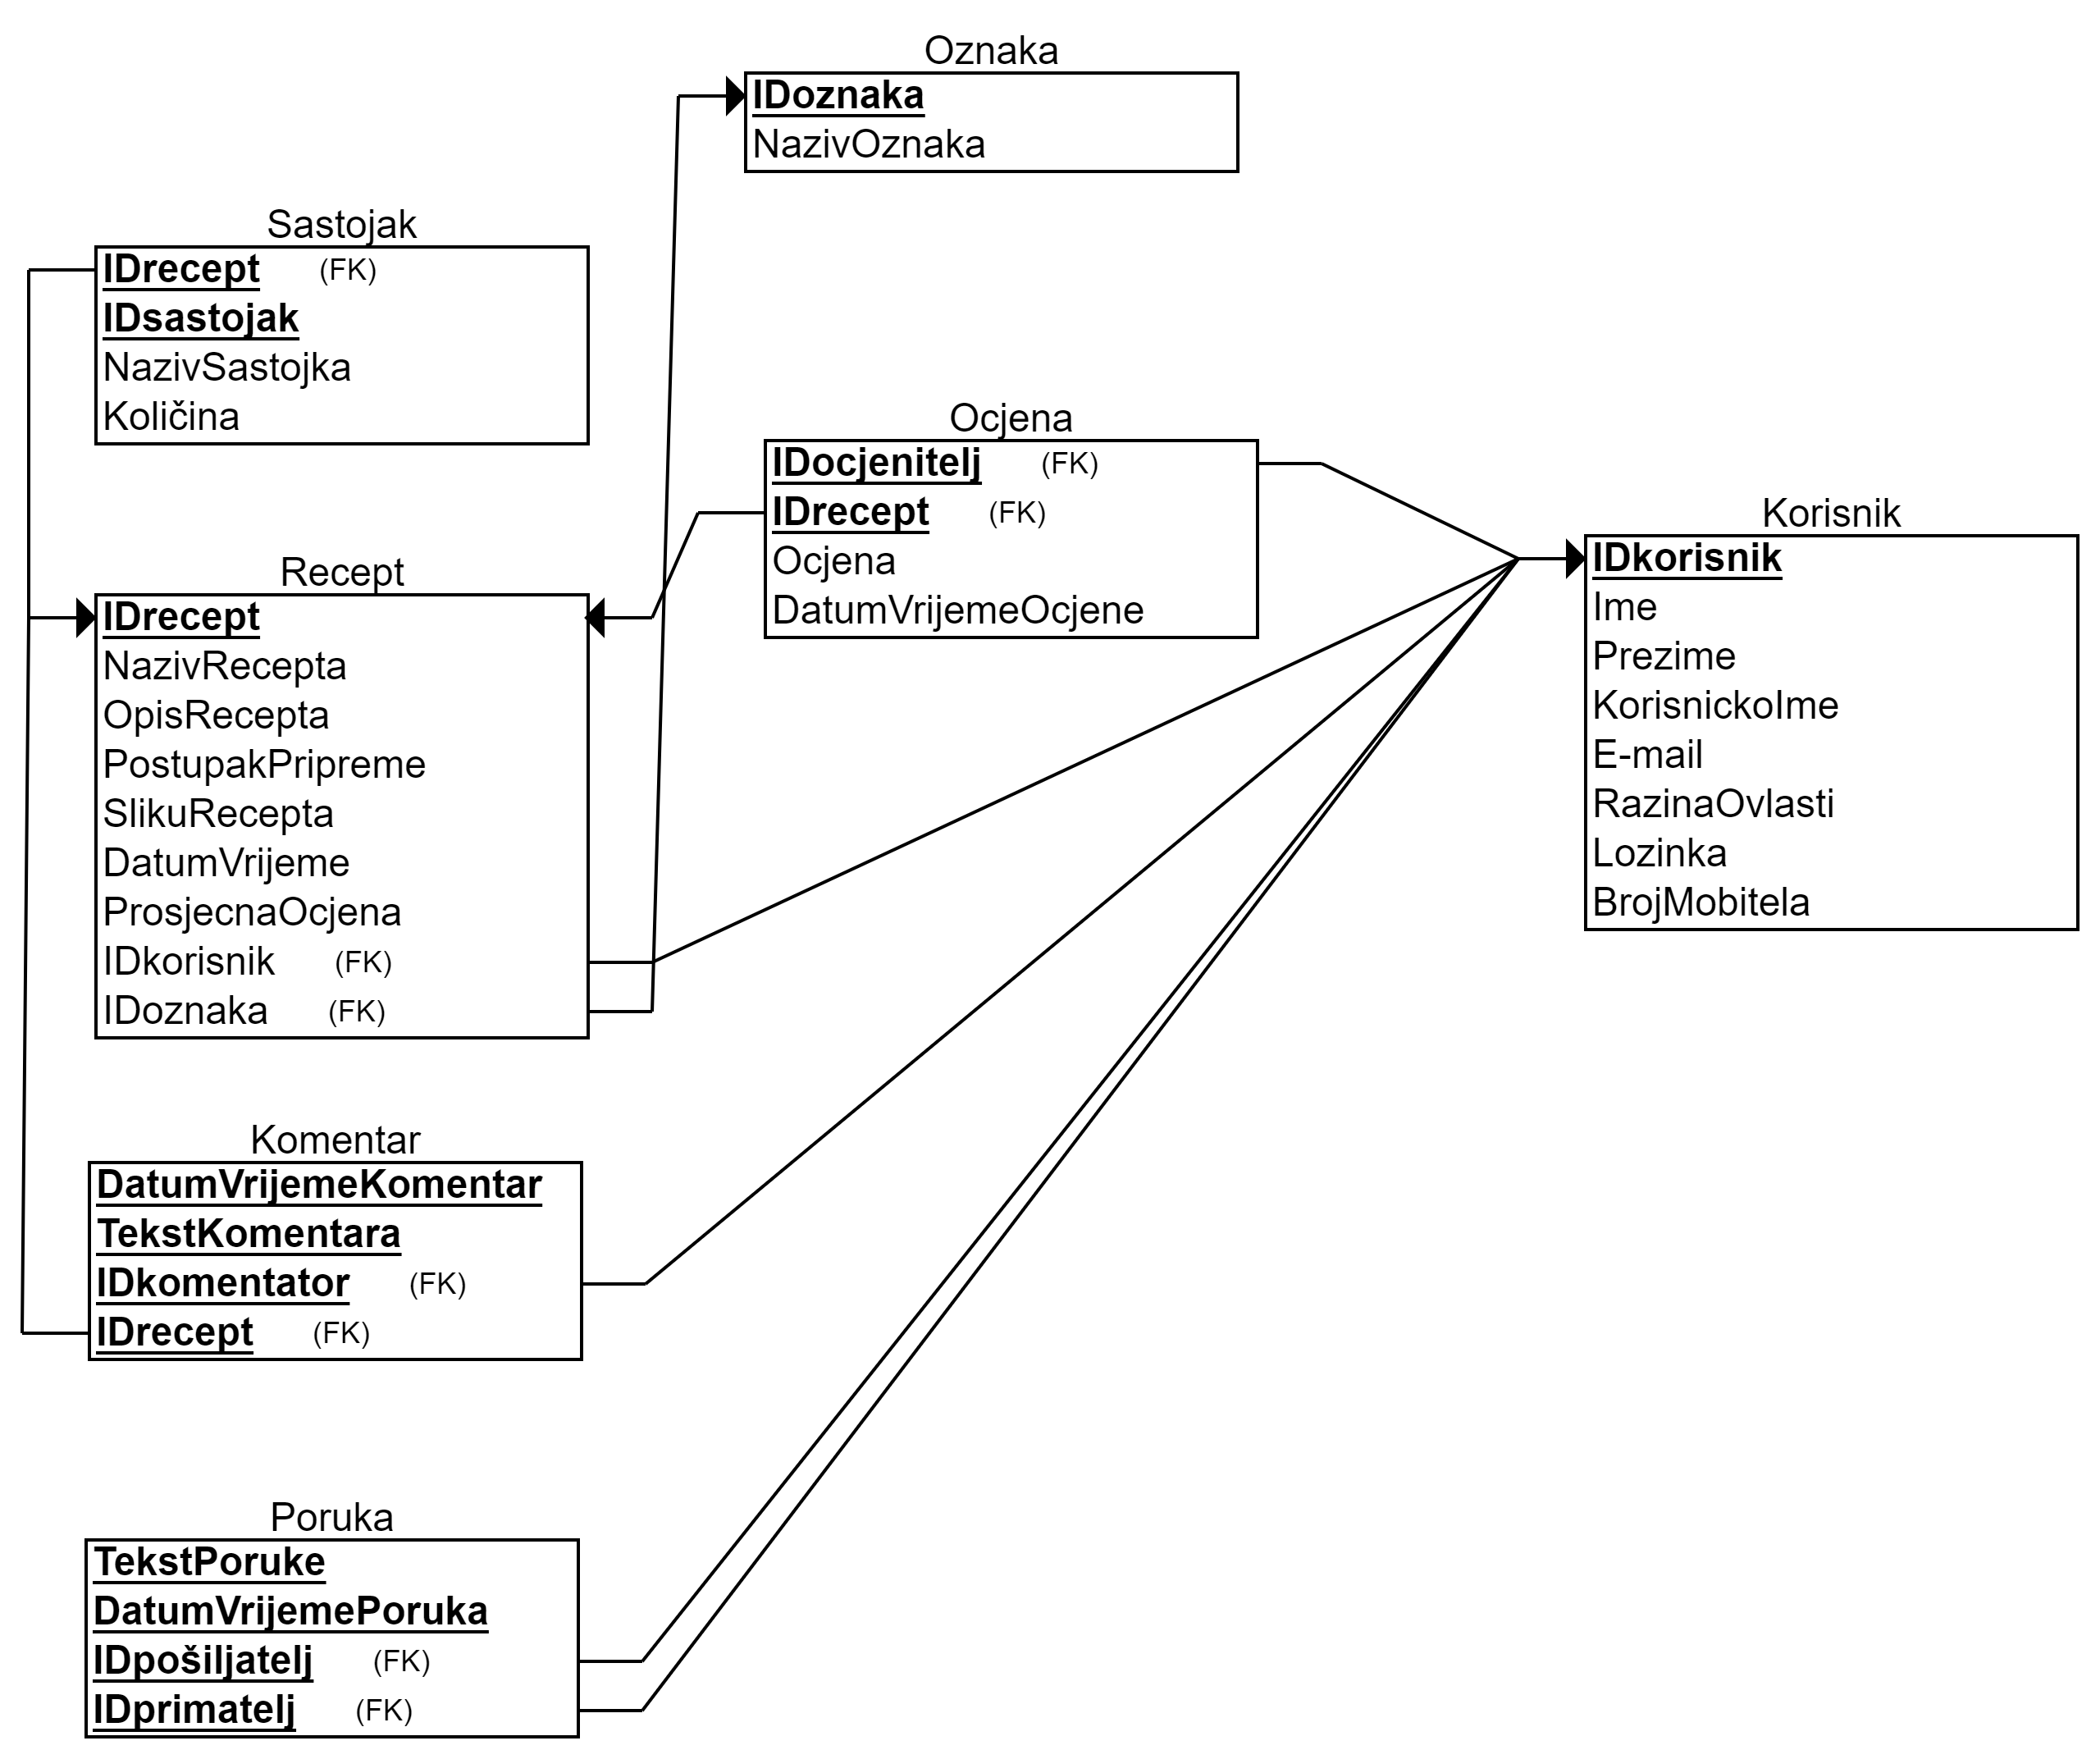
\includegraphics[scale=0.10]{slike/ER dijagram baze podataka.png} %veličina slike u odnosu na originalnu datoteku i pozicija slike
				 \centering
				 \caption{ER dijagram baze podataka}
				 \label{fig:ER dijagram baze podataka}
			 \end{figure}
		 
			 \eject
			
			
		\section{Dijagram razreda}

		Prvi dijagram prikazuje trenutno stanje stranice. Dijagram ima jedan repozitorij, entitet i servis te 5 kontrolera.
		\begin{figure}[H]
			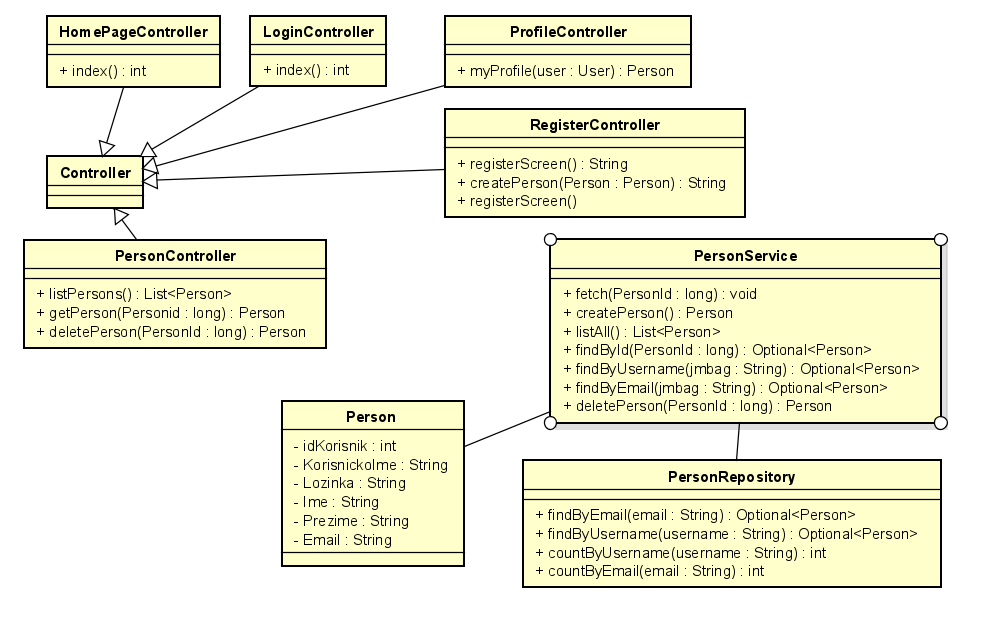
\includegraphics[scale=0.75]{slike/dijagram_razreda2.png} %veličina slike u odnosu na originalnu datoteku i pozicija slike
			\centering
			\caption{Dijagram razreda - dio Controllers}
			\label{fig:Dijagram_razreda2}
		\end{figure}


		Drugi dijagram prikazuje glavne entitete i veze između njih, 
		tj. preslikava strukturu baze podataka. Razred Korisnik 
		predstavlja neregistriranog korisnika koji se može registrirati 
		u Razred RegistriraniKorisnik predstavlja korisnika koji je registriran u sustav 
		i koji može koristiti više od osnovnih funkcija korisnika. NeRegistriraniKorisnik predstavlja vrstu korisnika i može se registrirati.
		Razred Administrator predstavlja administratora sustava koji ima najveće ovlasti. 



		\begin{figure}[H]
			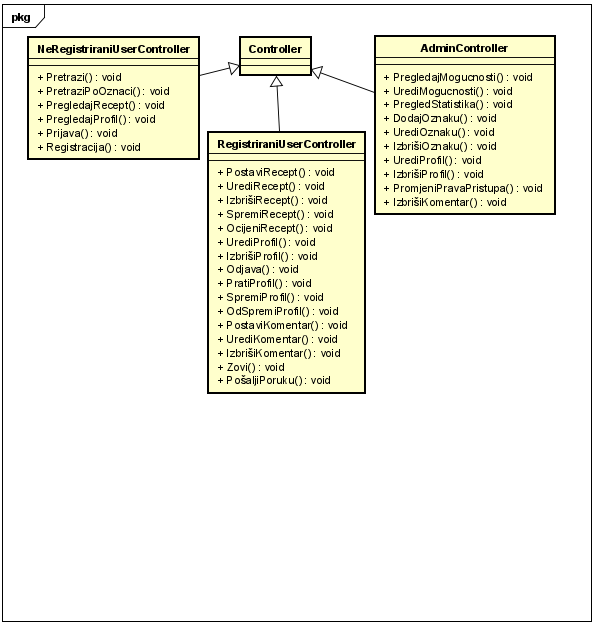
\includegraphics[scale=1.3]{slike/dijagram_razreda1.png} %veličina slike u odnosu na originalnu datoteku i pozicija slike
			\centering
			\caption{Dijagram razreda - dio Data transfer objects}
			\label{fig:Dijagram_razreda1}
		\end{figure}
			
			
			\eject
		
		\section{Dijagram stanja}
			
			
			% \textbf{\textit{dio 2. revizije}}\\
			
			% \textit{Potrebno je priložiti dijagram stanja i opisati ga. Dovoljan je jedan dijagram stanja koji prikazuje \textbf{značajan dio funkcionalnosti} sustava. Na primjer, stanja korisničkog sučelja i tijek korištenja neke ključne funkcionalnosti jesu značajan dio sustava, a registracija i prijava nisu. }
			Dijagram stanja na slici \ref{fig:Dijagram_stanja} opisuje stanja u kojima se registrirani korisnik može naći i njihove okidače te prijelaze. Nakon uspješne prijave, korisniku se prikazuje početna stranica na kojoj može pretražiti recept pomoću tražilice, pregledati svoj pretinac poruka, pregledati svoj profil, objaviti recept ili pogledati nove recepte koje su objavili korisnici koje prati. Na vlastitom profilu se prikazuju osobni podaci, objavljeni recepti i gumbovi za dodatne mogućnosti. Dodatne funkcionalnosti na stranici profila su opcije za daljnji pregled osobnih postavki, prikaz spremljenih recepata i prikaz korisnika koje prati. Klikom na "Postavke" korisnik može ažurirati svoje podatke ili obrisati svoj račun. Klikom na "Pretinac poruka" prikazuju se izmijenjene poruke. U pretincu se može otvoriti poruka njezinim odabirom te poslati nova poruka, čime se pritiskom gumba otvara šablona za poruku. Odabirom opcije "Objavi recept" otvara se nova stranica na kojoj se nalazi šablona za stvaranje recepta. Upisivanjem ključnih riječi u tražilicu prikaže se stranica s receptima koji se poklapaju s danim opisom. Odabirom recepta otvara se pojedinačna stranica sa samo odabranim receptom. Na stranici pregleda recepta korisnik može ocijeniti, spremiti ili komentirati recept, u slučaju da je korisnik autor prikazanog recepta pojavljuje se opcija uređivanja ili brisanja recepta. Korisnik također može pritisnuti na korisničko ime korisnika koji je objavio recept, time se otvara stranica tuđeg profila. Prikazivanjem tuđeg profila moguće je zapratiti korisnika ili poslati privatnu poruku korisniku, čime se ponovno otvara šablona za poruku. Korisnik uvijek ima mogućnost povratka na početnu stranicu, otvaranja pretinca poruka, pregleda korisničkog profila, pregleda novosti i objavljivanja recepta.
			\begin{figure}[H]
				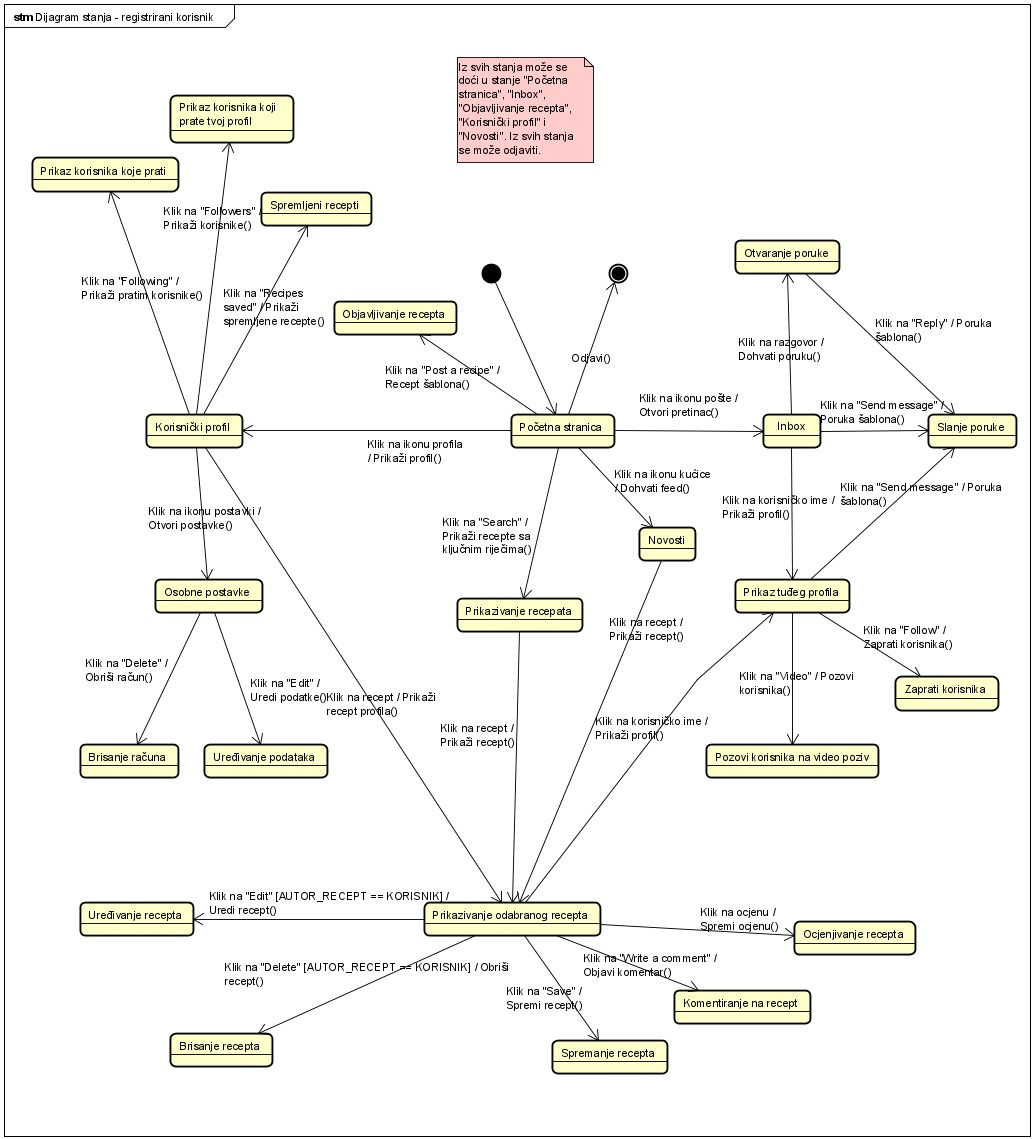
\includegraphics[scale=0.5]{slike/dijagram_stanja.jpeg} %veličina slike u odnosu na originalnu datoteku i pozicija slike
				\centering
				\caption{Dijagram stanja - registrirani korisnik}
				\label{fig:Dijagram_stanja}
			\end{figure}
			
			\eject 
		
		\section{Dijagram aktivnosti}
			
			%\textbf{\textit{dio 2. revizije}}\\
			
			 %\textit{Potrebno je priložiti dijagram aktivnosti s pripadajućim opisom. Dijagram aktivnosti treba prikazivati značajan dio sustava.}
			 Dijagram aktivnosti u nastavku prikazuje tok upravljanja jedne od najvažnijih funkcionalnosti stranice, a to je objava novog recepta. Dva glavna sudionika su korisnik koji objavljuje recept te baza podataka u koju se zapisuje, a cijelim postupkom upravlja sama aplikacija, odnosno back-end. Dijagram je sukladno tome podijeljen na tri particije.
			 
			 Korisnik se najprije mora prijaviti u aplikaciju. Nakon uspješne prijave prikazuje mu se početna stranica s koje korisnik može odabrati opciju za objavu novog recepta. Odabirom te opcije otvara se novi prozor te korisnik može započeti s pisanjem recepta. Nakon što je korisnik gotov s pisanjem, back-end provjerava sadrži li recept sve potrebne podatke. Ako je recept valjan, upisuje ga se u bazu podataka te se na kraju korisnicima koji prate autora u obliku poruke šalje obavijest o novoj objavi.
			 \begin{figure}
			 	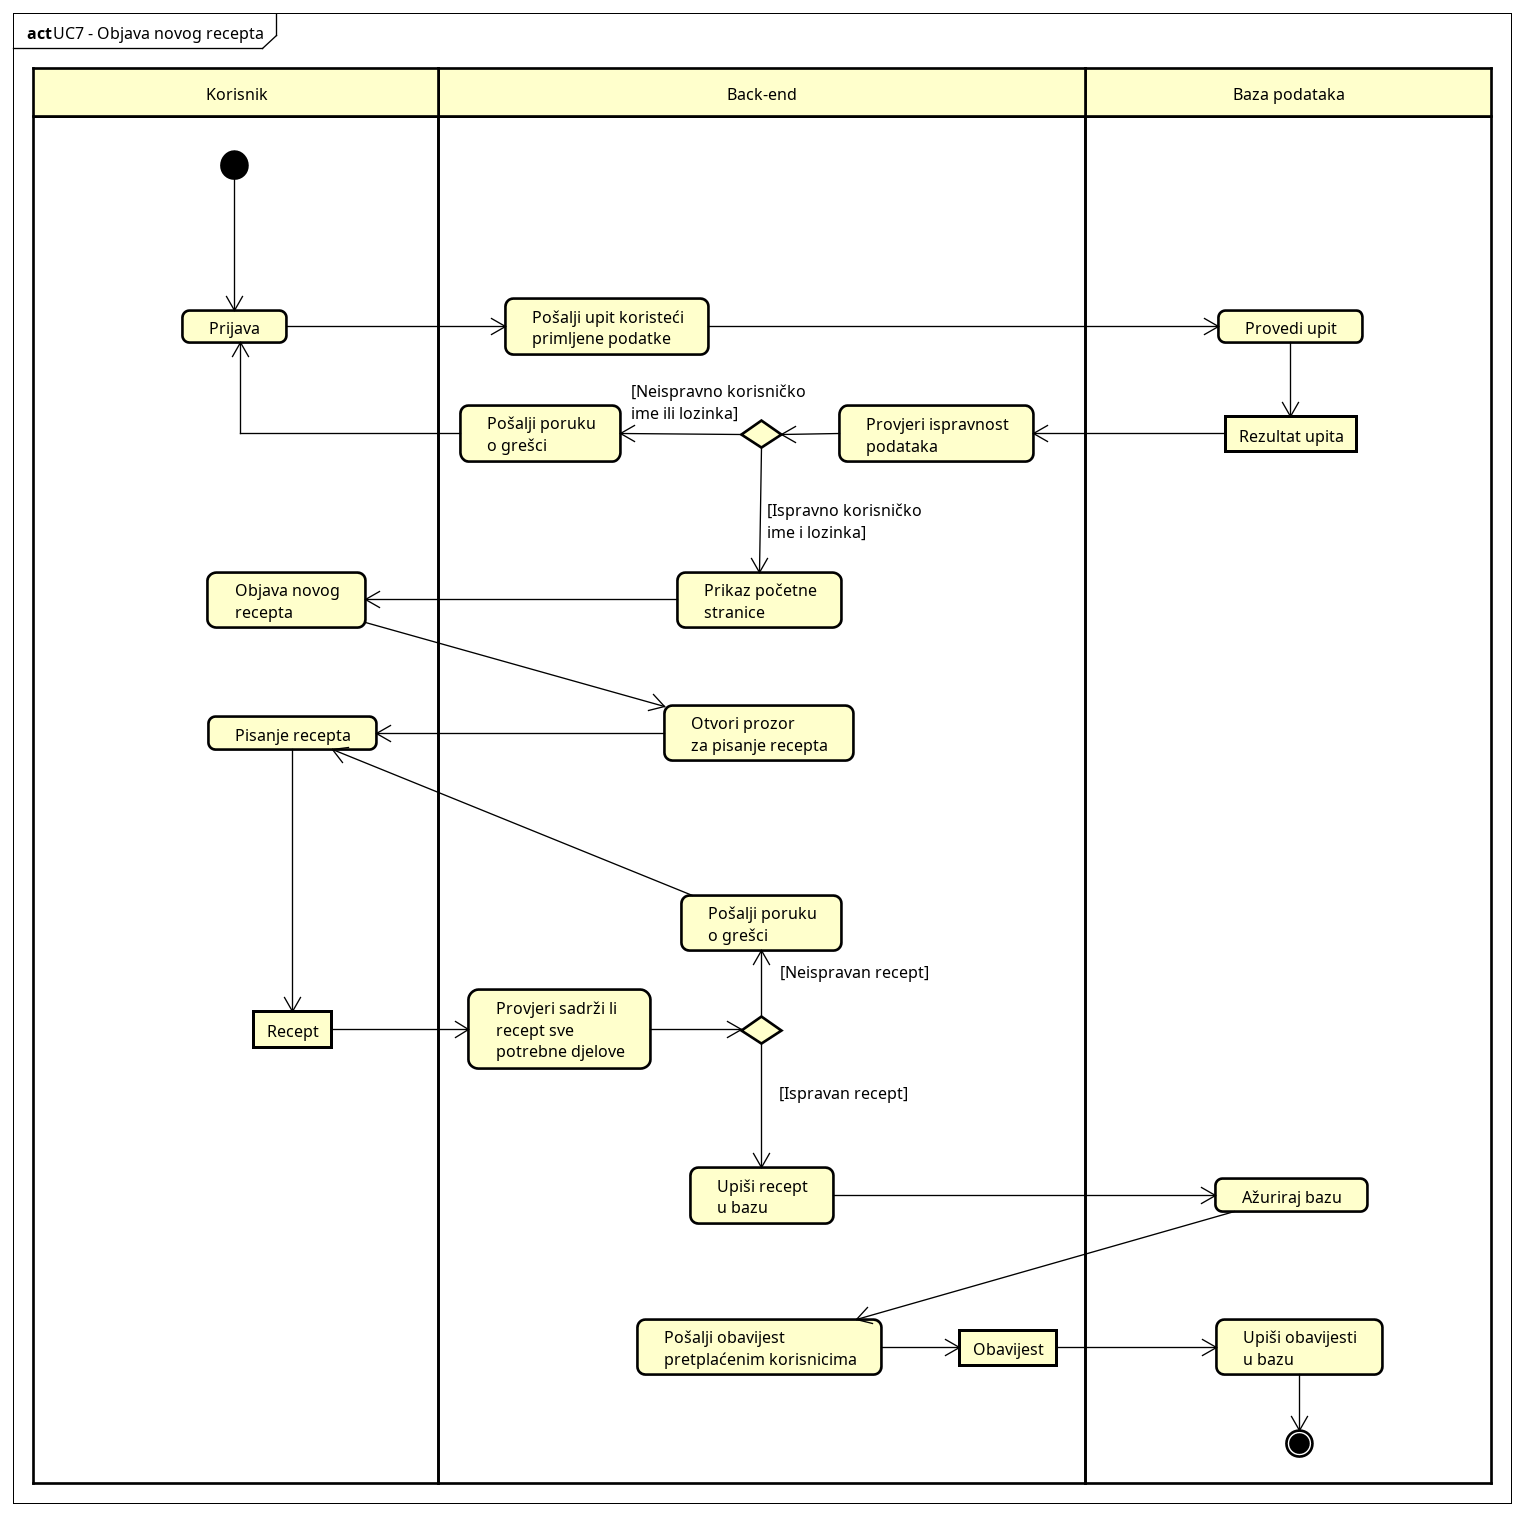
\includegraphics[scale=0.41]{slike/dijagram_aktivnosti.png}
			 	\centering
			 	\caption{Dijagram aktivnosti}
			 	\label{fig:Dijagram_aktivnosti}
			 \end{figure}
			 
			\eject
		\section{Dijagram komponenti}
		
			\textbf{\textit{dio 2. revizije}}\\
		
			 \textit{Potrebno je priložiti dijagram komponenti s pripadajućim opisom. Dijagram komponenti treba prikazivati strukturu cijele aplikacije.}